\documentclass[conference,onecolumn,11pt]{IEEEtran}
\IEEEoverridecommandlockouts
% The preceding line is only needed to identify funding in the first footnote. If that is unneeded, please comment it out.
\usepackage{cite}
\usepackage{amsmath,amssymb,amsfonts}
\usepackage{algorithmic}
\usepackage{graphicx}
\usepackage{textcomp}
\usepackage{xcolor}
\usepackage{booktabs} % for tables

\def\BibTeX{{\rm B\kern-.05em{\sc i\kern-.025em b}\kern-.08em
    T\kern-.1667em\lower.7ex\hbox{E}\kern-.125emX}}
\begin{document}

\title{Predicting Stock Market Volatility with Time Series Models\\
}

\author{\IEEEauthorblockN{1\textsuperscript{st} Xu Hao}
\IEEEauthorblockA{\textit{Department of Mathematics \& Statistics} \\
\textit{Thompson Rivers University}\\
Kamloops, Canada \\
xuh23@mytru.ca}
\and
\IEEEauthorblockN{2\textsuperscript{nd} Mulk Waqar Ul}
\IEEEauthorblockA{\textit{Department of Mathematics \& Statistics} \\
\textit{Thompson Rivers University}\\
Kamloops, Canada \\
mulkw22@mytru.ca}
}

\maketitle

\begin{abstract}
Predicting stock market movements is a significant challenge for traders, investors, and businesses, yet it can be highly profitable with precise forecasts. Achieving accurate predictions is crucial, particularly given the volatile, nonlinear, and unpredictable nature of the stock market. In this paper we are predicting stock prices of Apple using two machine learning algorithms - Linear Regression and Autoregressive Integrated Moving Average (ARIMA) by comparing their forecasting performances. The data is collected from Yahoo Finance and Google Trends and the analysis spans a period of eight years, from April 1st, 2016, to March 31st, 2024. The performance of the models are evaluated by root mean squared error (RMSE), mean squared error (MSE) and R-squared (R2). The findings of this study demonstrate that Simple Linear Regression is not well-suited for time series data analysis, whereas ARIMA presents distinct advantages in forecasting stock prices.

\end{abstract}

\begin{IEEEkeywords}
Forecasting, Stock Prices, Machine Learning, Autoregression, Linear Regression. 
\end{IEEEkeywords}

\section{Introduction}
A stock signifies an investment representing ownership in a company. The total ownership of a company is divided into shares, with each share representing an equal portion of the business. The stock market functions as a marketplace where individuals can purchase shares of stock. Analogous to various other markets like grocery stores or farmers’ markets, where multiple vendors gather to sell their products, the stock market serves as a central hub for trading securities. Similarly to a farmers’ market where different farmers offer their produce, customers have the opportunity to explore various investment options and make purchases according to their preferences. In essence, the stock market operates similarly to these markets, acting as a centralized venue where buyers and sellers converge to trade stocks and other investment instruments, including mutual funds, which pool together multiple stocks. However, unlike a single market, the stock market comprises several smaller markets known as stock exchanges.
Utilizing machine learning algorithms for stock price prediction aids in uncovering the potential future value of company stocks and other financial assets traded on various exchanges. The fundamental objective of predicting stock prices is to attain substantial profits. However, forecasting the performance of the stock market is a formidable challenge. Several factors come into play in this prediction process, encompassing both tangible and psychological elements, rational and irrational behaviors, among others.
The interaction of these diverse factors renders share prices highly dynamic and volatile, thereby posing significant hurdles to achieving precise predictions with a high degree of accuracy.


\subsection*{Linear Regression:}

Linear regression is a statistical method used to model the relationship between a dependent variable and one or more independent variables by fitting a linear equation to observed data. In essence, it seeks to determine the best-fitting straight line through the data points. The goal is to find the coefficients of the linear equation that minimize the difference between the observed and predicted values of the dependent variable. Linear regression is widely employed for prediction and forecasting tasks, as well as for understanding the relationships between variables in a dataset.

$Y = \beta_0+\beta_1 x_1 + \beta_2 x_2 + \ldots+\beta_n x_n + \epsilon$
y represents the dependent variable, x1, x2, ..., xn represents the independent variables, $\beta_0,\beta_1,\beta_2,\ldots,\beta_n$ represents the coefficients associated with each independent variable, and n is the number of independent variables. $\epsilon$represents the error term, which captures the difference between the observed and predicted values of the dependent variable.


\subsection*{ARIMA:}

ARIMA, or AutoRegressive Integrated Moving Average, is a forecasting algorithm grounded in the principle that historical values of a time series can offer insights into future trends. Belonging to a class of models renowned for elucidating time series behavior through its own past data, including lags and lagged forecast errors, ARIMA excels in predicting forthcoming values. It is particularly applicable to time series datasets exhibiting discernible patterns rather than random noise. ARIMA entails three key parameters: p, d, and q. The parameter p denotes the number of autoregressive terms or lag observations, providing lagged data points. d signifies the degree of differencing, indicating the number of times lagged indicators have been subtracted to achieve data stationarity. q represents the number of forecast errors in the model, akin to the size of the moving average window. These parameters, integers by nature, are pivotal in defining the ARIMA model's functionality and can take a value of 0, implying their exclusion from the model. Consequently, ARIMA can transform into various models: ARMA (p=0, d=0), AR (p$>$0, d=0, q=0), and MA (p=0, d=0, q$>$0). ARIMA models are denoted by their parameter combinations, such as ARIMA(1, 0, 0) for the first-order autoregressive model or ARIMA(0, 1, 0) for the random walk model. Once the parameters are set, the ARIMA model estimates coefficients $\alpha$ and $\theta$, utilizing past data points to forecast future values.

\section{Literature review}



\section{Data}
Data used for this paper is taken from Yahoo finance and Google Trend data. As we are only focused on Apple stocks data, we got the data only for Apple which ranges from April 1st, 2016 till March 31st, 2024. It consists of 6 independent variables and one response variable. The adjusted close price is a variable which we are using both as an independent and dependent variable. Table 1 shows statistics of the dataset that is used for training and testing.

\begin{table}[htbp]
    \centering
    \caption{Dataset Splitting}
    \begin{tabular}{@{}rlllll@{}}
        \toprule
         && \textbf{Dataset} & \textbf{Training} & \textbf{Validation} & \textbf{Testing} \\
        \midrule
        \textbf{Time Interval} &(Start) & 04-01-2016 & 04-01-2016 & 01-02-2021 & 07-01-2023\\
        &(End)& 03-31-2024 & 01-01-2021 & 06-30-2023 & 03-31-2024\\
  
        \bottomrule
    \end{tabular}
    \label{tab:GFS}
\end{table}

\begin{figure}[htpb]
	\centering
	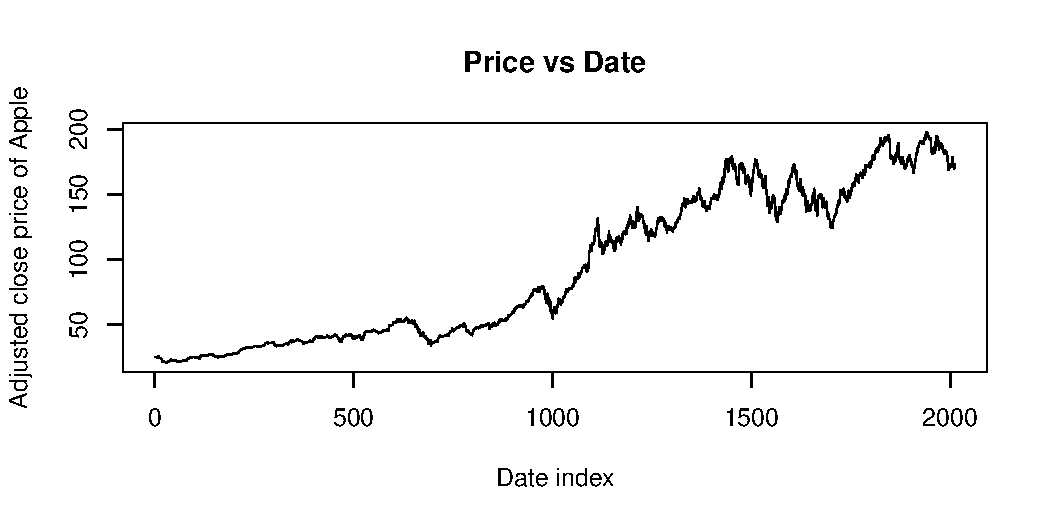
\includegraphics[width=0.8\textwidth]{pic/Price_vs_Date.pdf}
	\caption{}
	\label{fig:price}
\end{figure}

\begin{figure}[htpb]
	\centering
	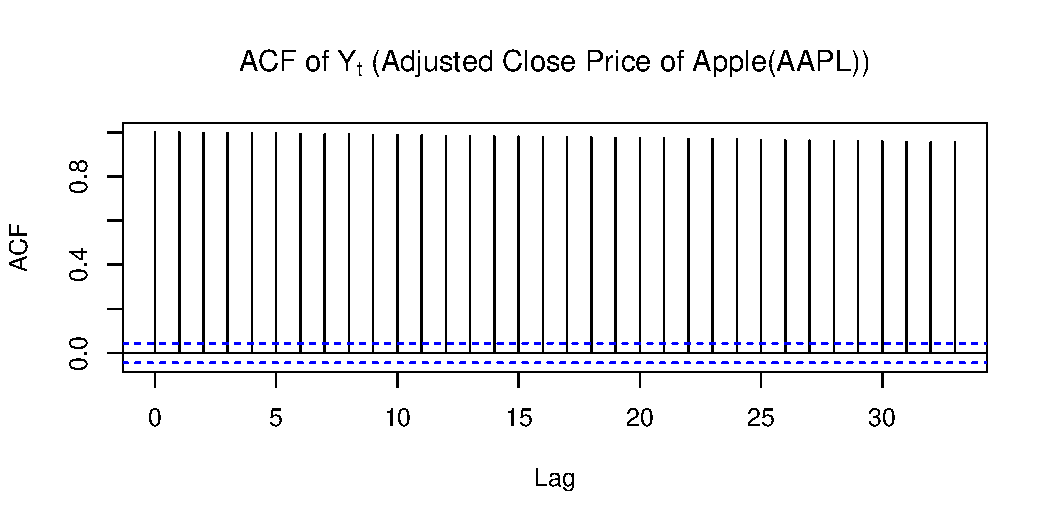
\includegraphics[width=0.8\textwidth]{pic/ACF_AdjClosed.pdf}
	\caption{}
	\label{fig:acf1}
\end{figure}

\begin{figure}[htpb]
	\centering
	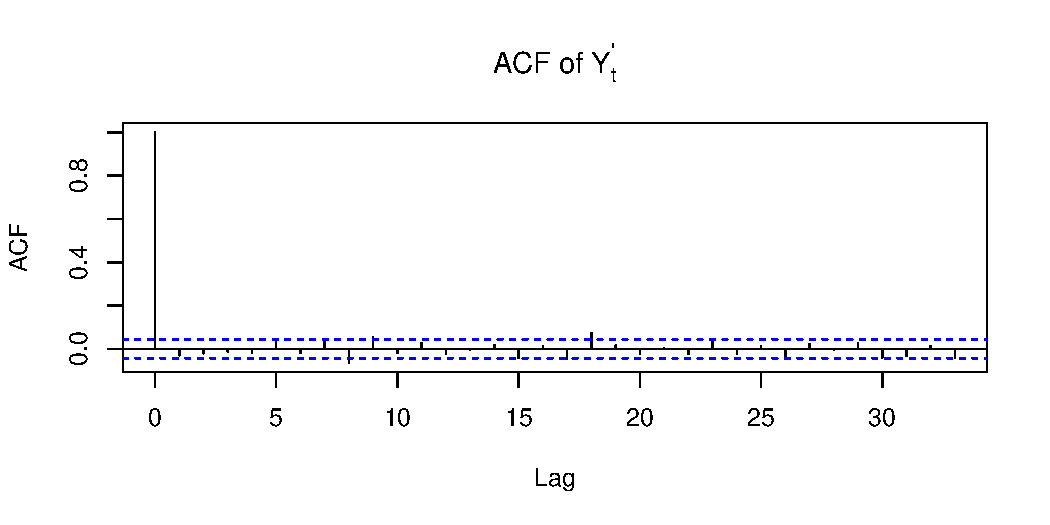
\includegraphics[width=0.8\textwidth]{pic/ACF_dAdjClosed.pdf}
	\caption{}
	\label{fig:acf2}
\end{figure}



\section{Method}

\subsection*{Univariate time series regression}

We use $y_{t}$ to represent the adjusted close price of Apple stock.
$y^{'}_{t} = \ln(y_{t})-\ln(y_{t-1}) = \ln(\frac{y_{t}}{y_{t-1}})$ represent the first difference of log of $y_{t}$.


Our AR($p$) model is defined as follows:

\[
y^{'}_{t} = c + \phi_{1}y^{'}_{t-1} + \phi_{2}y^{'}_{t-2} + \dots + \phi_{p}y^{'}_{t-p} + \varepsilon_{t},
\]

The predicted value for $y_t$ is calculated as follows:

\[
\hat{y}_t = \exp\{c + \phi_{1}y^{'}_{t-1} + \phi_{2}y^{'}_{t-2} + \dots + \phi_{p}y^{'}_{t-p}\}\cdot y_{t-1}
\]

\subsection*{Multivariate time series regression}



From Google trends, we get the interest over time of keywords ``Apple Watch", ``MacBook", ``AirPods", ``iPad", ``iPhone", represented by variable $y_{1,t},y_{2,t},y_{3,t},y_{4,t},y_{5,t}$ respectively. Also, we take the volume of the apple stock represented by variable $y_{6,t}$, the first difference of the adjusted close price of Apple stock as $y_{7,t}$ (which is $y^{'}_t$ in the univariate scenario). $\mathbf{y}_t = (y_{1,t},y_{2,t},y_{3,t},y_{4,t},y_{5,t},y_{6,t},y_{7,t})$.

We define our Vector Auto-Regressive(VAR) model as follows:

\[
\mathbf{y}_t = A_1\mathbf{y}_{t-1}+\ldots+A_p\mathbf{y}_{t-p}+\mathbf{u}_t
\]

where $A_i$ are $(7\times7)$ coefficient matrices for $i=1,\ldots,p$ and $\mathbf{u}_t$ is a 7-dimensional process with E($\mathbf{u}_t$) $= \mathbf{0}$ and time invariant positive definite covariance matrix E(${\mathbf{u}_t}{\mathbf{u}_t}^T$)$=\Sigma_\mathbf{u}$(white noise).



\section{Results}
\section{Discussion and/or Conclusion}

\section{Writing styles}

\begin{itemize}
\item Font: Times New Roman. The size of the font for the main body text must be 11 pt. 
\item One column. 
\item Single line spacing. 
\item Citations/references are to be done in Vancouver style. Citations are marked by a number in square brackets [1], which refers to a numbered reference in the references section. 
\item Sections should be clearly titled and numbered. 
\end{itemize}

\subsection{Equations}
Number equations consecutively. To make your 
equations more compact, you may use the solidus (~/~), the exp function, or 
appropriate exponents. Italicize Roman symbols for quantities and variables, 
but not Greek symbols. Use a long dash rather than a hyphen for a minus 
sign. Punctuate equations with commas or periods when they are part of a 
sentence, as in:
\begin{equation}
a+b=\gamma\label{eq}
\end{equation}

Be sure that the 
symbols in your equation have been defined before or immediately following 
the equation. Use ``\eqref{eq}'', not ``Eq.~\eqref{eq}'' or ``equation \eqref{eq}'', except at 
the beginning of a sentence: ``Equation \eqref{eq} is . . .''

\subsection{\LaTeX-Specific Advice}

Please use ``soft'' (e.g., \verb|\eqref{Eq}|) cross references instead
of ``hard'' references (e.g., \verb|(1)|). That will make it possible
to combine sections, add equations, or change the order of figures or
citations without having to go through the file line by line.

Please don't use the \verb|{eqnarray}| equation environment. Use
\verb|{align}| or \verb|{IEEEeqnarray}| instead. The \verb|{eqnarray}|
environment leaves unsightly spaces around relation symbols.

Please note that the \verb|{subequations}| environment in {\LaTeX}
will increment the main equation counter even when there are no
equation numbers displayed. If you forget that, you might write an
article in which the equation numbers skip from (17) to (20), causing
the copy editors to wonder if you've discovered a new method of
counting.

{\BibTeX} does not work by magic. It doesn't get the bibliographic
data from thin air but from .bib files. If you use {\BibTeX} to produce a
bibliography you must send the .bib files. 

{\LaTeX} can't read your mind. If you assign the same label to a
subsubsection and a table, you might find that Table I has been cross
referenced as Table IV-B3. 

{\LaTeX} does not have precognitive abilities. If you put a
\verb|\label| command before the command that updates the counter it's
supposed to be using, the label will pick up the last counter to be
cross referenced instead. In particular, a \verb|\label| command
should not go before the caption of a figure or a table.

Do not use \verb|\nonumber| inside the \verb|{array}| environment. It
will not stop equation numbers inside \verb|{array}| (there won't be
any anyway) and it might stop a wanted equation number in the
surrounding equation.

\subsection{Some Common Mistakes}\label{SCM}
\begin{itemize}
\item The word ``data'' is plural, not singular.
\item The subscript for the permeability of vacuum $\mu_{0}$, and other common scientific constants, is zero with subscript formatting, not a lowercase letter ``o''.
\item In American English, commas, semicolons, periods, question and exclamation marks are located within quotation marks only when a complete thought or name is cited, such as a title or full quotation. When quotation marks are used, instead of a bold or italic typeface, to highlight a word or phrase, punctuation should appear outside of the quotation marks. A parenthetical phrase or statement at the end of a sentence is punctuated outside of the closing parenthesis (like this). (A parenthetical sentence is punctuated within the parentheses.)
\item A graph within a graph is an ``inset'', not an ``insert''. The word alternatively is preferred to the word ``alternately'' (unless you really mean something that alternates).
\item Do not use the word ``essentially'' to mean ``approximately'' or ``effectively''.
\item In your paper title, if the words ``that uses'' can accurately replace the word ``using'', capitalize the ``u''; if not, keep using lower-cased.
\item Be aware of the different meanings of the homophones ``affect'' and ``effect'', ``complement'' and ``compliment'', ``discreet'' and ``discrete'', ``principal'' and ``principle''.
\item Do not confuse ``imply'' and ``infer''.
\item The prefix ``non'' is not a word; it should be joined to the word it modifies, usually without a hyphen.
\item There is no period after the ``et'' in the Latin abbreviation ``et al.''.
\item The abbreviation ``i.e.'' means ``that is'', and the abbreviation ``e.g.'' means ``for example''.
\end{itemize}
An excellent style manual for science writers is \cite{b7}.


\subsection{Figures and Tables}
\paragraph{Positioning Figures and Tables} Place figures and tables at the top and bottom of columns. Avoid placing them in the middle of columns. Large figures and tables may span across both columns. Figure captions should be below the figures; table heads should appear above the tables. Insert figures and tables after they are cited in the text. Use the abbreviation ``Fig.~\ref{fig}'', even at the beginning of a sentence.

\begin{table}[htbp]
\caption{Table Type Styles}
\begin{center}
\begin{tabular}{|c|c|c|c|}
\hline
\textbf{Table}&\multicolumn{3}{|c|}{\textbf{Table Column Head}} \\
\cline{2-4} 
\textbf{Head} & \textbf{\textit{Table column subhead}}& \textbf{\textit{Subhead}}& \textbf{\textit{Subhead}} \\
\hline
copy& More table copy$^{\mathrm{a}}$& &  \\
\hline
\multicolumn{4}{l}{$^{\mathrm{a}}$Sample of a Table footnote.}
\end{tabular}
\label{tab1}
\end{center}
\end{table}

\begin{figure}[htbp]
\centerline{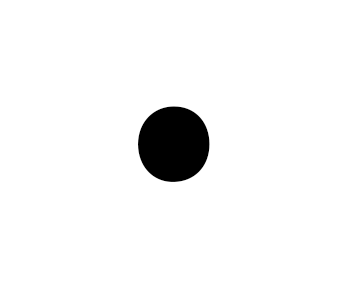
\includegraphics{fig1.png}}
\caption{Example of a figure caption.}
\label{fig}
\end{figure}

Figure Labels: Use 8 point Times New Roman for Figure labels. Use words 
rather than symbols or abbreviations when writing Figure axis labels to 
avoid confusing the reader. As an example, write the quantity 
``Magnetization'', or ``Magnetization, M'', not just ``M''. If including 
units in the label, present them within parentheses. Do not label axes only 
with units. In the example, write ``Magnetization (A/m)'' or ``Magnetization 
\{A[m(1)]\}'', not just ``A/m''. Do not label axes with a ratio of 
quantities and units. For example, write ``Temperature (K)'', not 
``Temperature/K''.

\section*{References}

Please number citations consecutively within brackets \cite{b1}. The 
sentence punctuation follows the bracket \cite{b2}. Refer simply to the reference 
number, as in \cite{b3}---do not use ``Ref. \cite{b3}'' or ``reference \cite{b3}'' except at 
the beginning of a sentence: ``Reference \cite{b3} was the first $\ldots$''

Number footnotes separately in superscripts. Place the actual footnote at 
the bottom of the column in which it was cited. Do not put footnotes in the 
abstract or reference list. Use letters for table footnotes.

Unless there are six authors or more give all authors' names; do not use 
``et al.''. Papers that have not been published, even if they have been 
submitted for publication, should be cited as ``unpublished'' \cite{b4}. Papers 
that have been accepted for publication should be cited as ``in press'' \cite{b5}. 
Capitalize only the first word in a paper title, except for proper nouns and 
element symbols.

For papers published in translation journals, please give the English 
citation first, followed by the original foreign-language citation \cite{b6}.

\begin{thebibliography}{00}
\bibitem{b1} Selene Yue Xu. (n.d.). https://www.econ.berkeley.edu/sites/default/files/Selene%20Yue%20Xu.pdf
\bibitem{b2} Khanderwal, S., & Mohanty, D. (2021). Stock Price Prediction Using ARIMA Model. International Journal of Marketing & Human Resource Research, 2(2), 98-107. Retrieved from http://www.journal.jis-institute.org/index.php/ijmhrr/article/view/235
\bibitem{b3} Vijh, M., Chandola, D., Tikkiwal, V. A., & Kumar, A. (2020). Stock Closing Price Prediction using Machine Learning Techniques. Procedia Computer Science, 167(167), 599–606. https://doi.org/10.1016/j.procs.2020.03.326

\bibitem{b4} K. Elissa, ``Title of paper if known,'' unpublished.
\bibitem{b5} R. Nicole, ``Title of paper with only first word capitalized,'' J. Name Stand. Abbrev., in press.
\bibitem{b6} Y. Yorozu, M. Hirano, K. Oka, and Y. Tagawa, ``Electron spectroscopy studies on magneto-optical media and plastic substrate interface,'' IEEE Transl. J. Magn. Japan, vol. 2, pp. 740--741, August 1987 [Digests 9th Annual Conf. Magnetics Japan, p. 301, 1982].
\bibitem{b7} M. Young, The Technical Writer's Handbook. Mill Valley, CA: University Science, 1989.
\end{thebibliography}
\vspace{12pt}
\end{document}
